
%\documentclass[calculator,steamtables,refrigeranttables,psychrometricchart,datasheet,solutions]{exam}
\documentclass[calculator,steamtables,refrigeranttables,psychrometricchart,datasheet,sample]{exam}

% The full list of class options are
% calculator : Allows approved calculator use.
% datasheet : Adds a note that data sheet are attached to the exam.
% handbook : Allows the use of the engineering handbook.
% resit : Adds the resit markings to the paper.
% sample : Adds conspicuous SAMPLE markings to the paper
% solutions : Uses the contents of \solution commands (and \solmarks) to generate a solution file

\usepackage{pdfpages}
\usepackage{lscape,comment}

\coursecode{EG3521}%%
\coursetitle{Engineering Thermodynamics}%
%\coursecode{EG3539}%
%\coursetitle{Thermodynamics}%

\examtime{00.00--00.00}%
\examdate{00}{05}{2014}%
\examformat{Candidates must attempt \textit{all} questions.}

\newcommand{\frc}{\displaystyle\frac}
\newcommand{\br}[1]{\!\left( #1 \right)}
\newcommand{\abs}[1]{\left| #1 \right|}
\newcommand{\fracd}[2]{\frac{\mathrm{d} #1}{\mathrm{d} #2}}
\newcommand{\fracp}[2]{\frac{\partial #1}{\partial #2}}
\renewcommand{\d}[1]{\mathrm{d} #1 }
\newcommand{\Ma}{\mathrm{M\!a}}



\begin{document}

%%%
%%% Question 01
%%%
\begin{question}

An engine operates in a {\it dual cycle} with compression $\left(r_{c}\right)$ and expansion $\left(r_{e}\right)$ ratios of 9 and 5, respectively. The initial pressure and temperature of the air are 1 bar and 30$^{\text{o}}$C. The heat liberated at constant pressure is twice the heat liberated at constant volume, i.e.,
\begin{displaymath}
C_{p}\left(T_{4}-T_{3}\right)=2 C_{v}\left(T_{3}-T_{2}\right).
\end{displaymath}
The isentropic expansion and compression strokes follow $PV^{n}=\text{ constant}$, with $n=1.25$. The cylinder bore (diameter) is of 250 mm and the stroke length is of 400 mm. 
\begin{enumerate}[(a)]

%%%
%%%
%%%
\item Calculate pressures and temperatures at all strokes and fill up the table below,
\begin{center}
\begin{tabular}{||c |c |c ||}
\hline \hline
 {\bf Stroke}  &  {\bf P (bar)}   &  {\bf T (K)} \\
\hline\hline
{\bf 1 }       &     1.0          &    303.15    \\
\hline         
{\bf 2 }       &                  &             \\
\hline         
{\bf 3 }       &                  &             \\
\hline         
{\bf 4 }       &                  &             \\
\hline         
{\bf 5 }       &                  &             \\
\hline\hline         
\end{tabular}
\end{center}
\begin{flushright}
{\bf [8 Marks]}
\end{flushright}
%%%
%%%
%%%



%%%
%%%
%%%
\item Sketch the {\it P-v} diagram for this cycle, indicating the swept $\left(V_{s}\right)$ and TDC $\left(V_{c}\right)$ volumes.
\begin{flushright}
{\bf [2 Marks]}
\end{flushright} 

%%%
%%%
%%%
\item Calculate the Mean Effective Pressure (MEP) of the cycle (in bar) using the following expression:
\begin{displaymath}
MEP = \frc{1}{r_{c}-1} \left[ P_{3}\left(\rho-1\right) + \frc{P_{4}\rho-P_{5}r_{c}}{n-1} - \frc{P_{2}-P_{1}r_{c}}{n-1}\right]
\end{displaymath}
\begin{flushright}
{\bf [2 Marks]}
\end{flushright}

%%%
%%%
%%%
\item Calculate {\it work done per cycle} (in kJ) and the {\it heat supplied per cycle} (in kJ), given by
\begin{displaymath}
W_{\text{cycle}} = MEP \times V_{s} \;\;\;\;{\text and } \;\;\;\; Q_{\text{cycle}} = m Q_{s} = m \left[ C_{p}\left(T_{3}-T_{2}\right) + C_{p}\left(T_{4}-T_{3}\right)\right]  
\end{displaymath}
Given: $V_{1}=V_{s}+V_{c}=\frc{r_{c}}{r_{c}-1}V_{s}$
\begin{flushright}
{\bf [2 Marks]}
\end{flushright}

%%%
%%%
%%%
\item Sketch {\it T-S} and {\it P-V} diagrams for the Otto and Diesel cycles.
\begin{flushright}
{\bf [6 Marks]}
\end{flushright} 
%
\end{enumerate}

Also given: 
\begin{eqnarray}
&& C_{p}=1.0\frc{\text{kJ}}{\text{kg.K}}\;,\;\;C_{v}=0.71\frc{\text{kJ}}{\text{kg.K}}\;, \;\; MW=29 \frc{\text{g}}{\text{gmol}}\;\; \text{(molecular weight),} \nonumber \\
&& R=8.3144621\times 10^{-5}\frc{\text{m}^{3}.\text{bar}}{\text{K.gmol}}\;\;\text{(gas constant),}\;\; \rho = \frc{r_{c}}{r_{e}} \nonumber 
\end{eqnarray}

\end{question}

\clearpage


%%%
%%% Question 2
%%%
\begin{question}\vspace{-2\baselineskip}

\begin{enumerate}[(a)]
%
\item A horizontally mounted turbine is housed between circular inlet and outlet pipes of circumference 1 m and 0.6 m, respectively. Assume gas satisfying the steady flow energy conservation
\begin{displaymath}
\frc{ \dot{Q} -\dot{W}_{s}}{\dot{m}} = \left( h_{2}+ \frc{u_{2}^{2}}{2}\right) - \left(h_{1} + \frc{u_{1}^{2}}{2}\right),
\end{displaymath}
flows through the turbine at a steady rate of 4 kg/s. At the inlet (labelled 1), the fluid has a specific enthalpy $h$ of 70 kJ/kg and a velocity $u$ of 30 m/s, while at the outlet (labelled 2), the fluid has a specific enthalpy of 40 kJ/kg. If the gas does work on the turbine at a rate of 30 kW and transfers heat to the surroundings at a rate of 15 kW, then find the change in gas density between the inlet and the outlet. {\bf [4 Marks]}

%
\item For gas flow along a duct whose length is parameterized by $x$ and has slowly-varying cross-sectional area  $A(x)$, use equations corresponding to mass and energy conservation to show that
\begin{displaymath}
\frc{dV}{V} + \frc{d h}{u^{2}} - \frc{dA}{A}=0,
\end{displaymath}
where the specific volume is denoted $V$, the specific enthalpy $h$, and fluid velocity $u$. {\bf [2 Marks]}
\medskip

\item Define the speed of sound $c$ and the Mach number $M\! a$ in a gas. State equations that are appropriate for calculating these quantities in an isentropic gas and define the variables used. {\bf [4 Marks]}
\medskip

\item For an isentropic process show that changes in specific volume are related to changes in pressure ($p$) through
\begin{displaymath}
dV=-\frc{V^{2}}{c^{2}}dp,
\end{displaymath}
and explain how changes in specific enthalpy are related to changes in pressure. {\bf [3 Marks]}
\medskip

\item Hence, for isentropic flow along a duct, show that
\begin{displaymath}
\frc{1}{A\left(1- M\! a^{2}\right)}\frc{dA}{dx} = \frc{1}{\rho \, M\! a^{2}}\frc{d\rho}{dx},
\end{displaymath}
where the gas density is denoted $\rho$. {\bf [5 Marks]}
\medskip

\item Explain with reasoning how the gas density changes for flow along a supersonic diffuser. {\bf [2 Marks]}
%
\end{enumerate}

\end{question}


\clearpage


%%%
%%% Question 3
%%%
\begin{question} \vspace{-2\baselineskip}
\begin{enumerate}[(a)] 
\item Define the specific humidity $\omega$, the saturation pressure of water vapour $p_{\text{v,sat}}$, and relative humidity $\varphi$. Assuming that dry air and water vapour behave like ideal gases show that
\begin{displaymath}
\omega = \frc{R_{a}\varphi p_{\text{v,sat}}}{R_{v}\left(p - \varphi p_{\text{g,v,sat}}\right)},
\end{displaymath}
where $R_{a}$ and $R_{v}$ are the specific gas constants of dry air and water vapour, respectively. 
\begin{flushright}
{\bf [5 Marks]}
\end{flushright} 

\item Air leaving an air-conditioning system in a building is mixed adiabatically with air from outside in a steady process. If the inlets to the mixing chamber are labelled 1 and 2 and the outlet is labelled 3, then state equations corresponding to the mass conservation of dry air, the mass conservation of water vapour and the conservation of energy. Hence show that
\begin{displaymath}
\frc{\dot{m}_{a2}}{\dot{m}_{a1}} = \frc{\omega_{}-\omega_{1}}{\omega_{2}-\omega_{3}} = \frc{h_{3}-h_{1}}{h_{2}-h_{3}}
\end{displaymath}
where $\dot{m}_{a}$  is a mass flux of dry air and $h$ is an enthalpy.
\begin{flushright}
{\bf [7 Marks]}
\end{flushright} 

\item Saturated air at 16$^{\text{o}}$C leaves the cooling section of an air-conditioning system in a building at a rate of 1 m$^{3}$/s. This air is mixed adiabatically at a constant pressure of 100 kPa, with air from outside that has temperature 30$^{\text{o}}$C and specific humidity 0.0182 kg H$_{2}$O/kg dry air. If the mass flux of dry air after mixing is 1.8 kg/s, then:
\begin{enumerate}[(i)]
\item Determine the mass flux through both inlets;
\begin{flushright}
{\bf [3 Marks]}
\end{flushright} 
\item Calculate the specific humidity of the air leaving the cooling section of the air-conditioning system;
\begin{flushright}
{\bf [1 Mark]}
\end{flushright} 
\item Calculate the specific humidity of the mixed air. 
\begin{flushright}
{\bf [4 Marks]}
\end{flushright} 
\end{enumerate}
\end{enumerate}
You may assume the saturation pressure of water vapour at 16$^{\text{o}}$C is 1818.747 Pa and that the specific gas constants $R_{a}=287.1$ J/(kg.K) and $R_{v}=461.5$ J/(kg.K), respectively.
\end{question}


\clearpage



%%%(saphiro 10.17)
%%% Question 4 
%%%
\begin{question} A vapour-compression refrigeration system circulates Refrigerant 134a at a rate of 6 kg/min. The refrigerant enters the compressor at -10$^{\text{o}}$C, 1.4 bar and exits at 7 bar. The isentropic compressor efficiency is 67$\%$. There are no appreciable pressure drops as the refrigerant flows through the condenser and evaporator. The refrigerant leaves the condenser at 7 bar, 24$^{o}$C. Ignoring heat transfer between the compressor and its surroundings, determine:
\begin{enumerate}[(a)]
\item $H_{i}$, $i\in\{1,2,3,4\}$;
\begin{flushright}
{\bf [8 Marks]}
\end{flushright} 
\item Coefficient of performance, $\beta$;
\begin{displaymath}
\beta = \frc{H_{1}-H_{4}}{H_{2}-H_{1}}
\end{displaymath}
\begin{flushright}
{\bf [3 Marks]}
\end{flushright} 
\item Refrigeration capacity, $\dot{Q}_{\text{in}}$ (in ton),
\begin{displaymath}
\dot{Q}_{\text{in}}=\dot{m}\left(H_{1}-H_{4}\right)
\end{displaymath}
\begin{flushright}
{\bf [3 Marks]}
\end{flushright} 
\item Sketch the schematics of the process and {\it T-S} diagram for this cycle.
\begin{flushright}
{\bf [6 Marks]}
\end{flushright} 
\end{enumerate}
In the expressions above for $\beta$ and $\dot{Q}_{\text{in}}$, assume that subscripts $1$, $2$, $3$ and $4$ represent the following flows:
\begin{itemize}
\item $1$: Evaporator $\Rightarrow$ Compressor; 
\item $2$: Compressor $\Rightarrow$ Condenser; 
\item $3$: Condenser $\Rightarrow$  Expansion Valve and; 
\item $4$: Expansion Valve $\Rightarrow$   Evaporator.
\end{itemize}
Also given: {\it 1 ton} = $1.4\times 10^{4}\;\;\frc{kJ}{h}$
\end{question}

\clearpage


%%%
%%% Question 05
%%%
\begin{question} 
In the secondary cooling circuit of a nuclear power plant, the steam generator (boiler / reheater) is connected to two turbines operating as a reheat Rankine cycle (Fig. \ref{exam_mod01_rankinecycle}). Primary superheated steam is at 40 bar and 370$^{\text{o}}$C, with reheat to 7 bar and 370$^{\text{o}}$C. The isentropic efficiencies of the first $\left(\eta_{\text{T1}}\right)$ and second $\left(\eta_{\text{T2}}\right)$ turbines and boiler feed pump $\left(\eta_{\text{P}}\right)$ are 84$\%$, 80$\%$ and 61$\%$ respectively. 

\begin{figure}[h]
\begin{center}
\includegraphics[width=15.cm,clip]{./Pics/Exam_Reheat_Rankine_Cycle}
\caption{ Reheat Rankine cycle with 2 turbines.}
\label{exam_mod01_rankinecycle}
\end{center}
\end{figure}


\begin{enumerate}[(a)]
\item In the Table below, determine {\it (a)-(j)}. {\bf [10 Marks]}\\
%\begin{table}[h]
%\label{exam1_table1}
\begin{center}
\begin{tabular} {||c | c c c c c || }
\hline\hline
{\bf Stage} & {\bf P}    & {\bf T}        & {\bf State}    & {\bf H}             & {\bf S}                  \\
            & {\bf (bar)}& {\bf ($^{o}$C)} &               & {\bf (kJ.kg$^{-1}$)} & {\bf (kJ.(kg.K)$^{-1}$)} \\
\hline\hline
 {\bf 1 }   & 40         & 370            &   superheated  & {\bf (a)}           & {\bf (b)}                 \\
            &            &                &   steam        &                     &                           \\
 {\bf 2 }   &  --        &  --            &     {\bf (c)}  & --                  &   --                      \\
 {\bf 3 }   & 7          & 370            &   superheated  & {\bf (d)}           & {\bf (e)}                 \\
            &            &                &   steam        &                     &                           \\
 {\bf 4 }   & 0.10       & --             &     --         & --                   & --                      \\
 {\bf 5 }   & 0.10       & --             &   {\bf (f)}    & {\bf (g)}           & {\bf (h)}                 \\
 {\bf 6 }   & 40         & --             &   {\bf (i)}    & {\bf (j)}           & --                       \\

\hline\hline
\end{tabular}
\end{center}
%\caption{Thermodynamic table of the reheat Rankine cycle.}
%\end{table}


\item Calculate the thermal efficiency $\left(\eta_{\text{Thermal}}\right)$ of the reheat Rankine cycle with 2 turbines. $\eta_{\text{Thermal}}$ is expressed as, 
\begin{displaymath}
\eta_{\text{Thermal}} = \frc{ \left(H_{1}-H_{2s}\right)\eta_{\text{T1}} + \left(H_{3}-H_{4s}\right)\eta_{\text{T2}} - V_{5}\left(P_{6}-P_{5}\right)\eta_{\text{P}}^{-1}} {\left(H_{1}-H_{6}\right)+\left(H_{3}-H_{2}\right)}
\end{displaymath}
where the subscript {\it s} indicates the ideal state. {\bf [5 Marks]}

\item Sketch the {\it T-S} diagram for this cycle. {\bf [5 Marks]}

\end{enumerate}

\end{question}

\clearpage

{
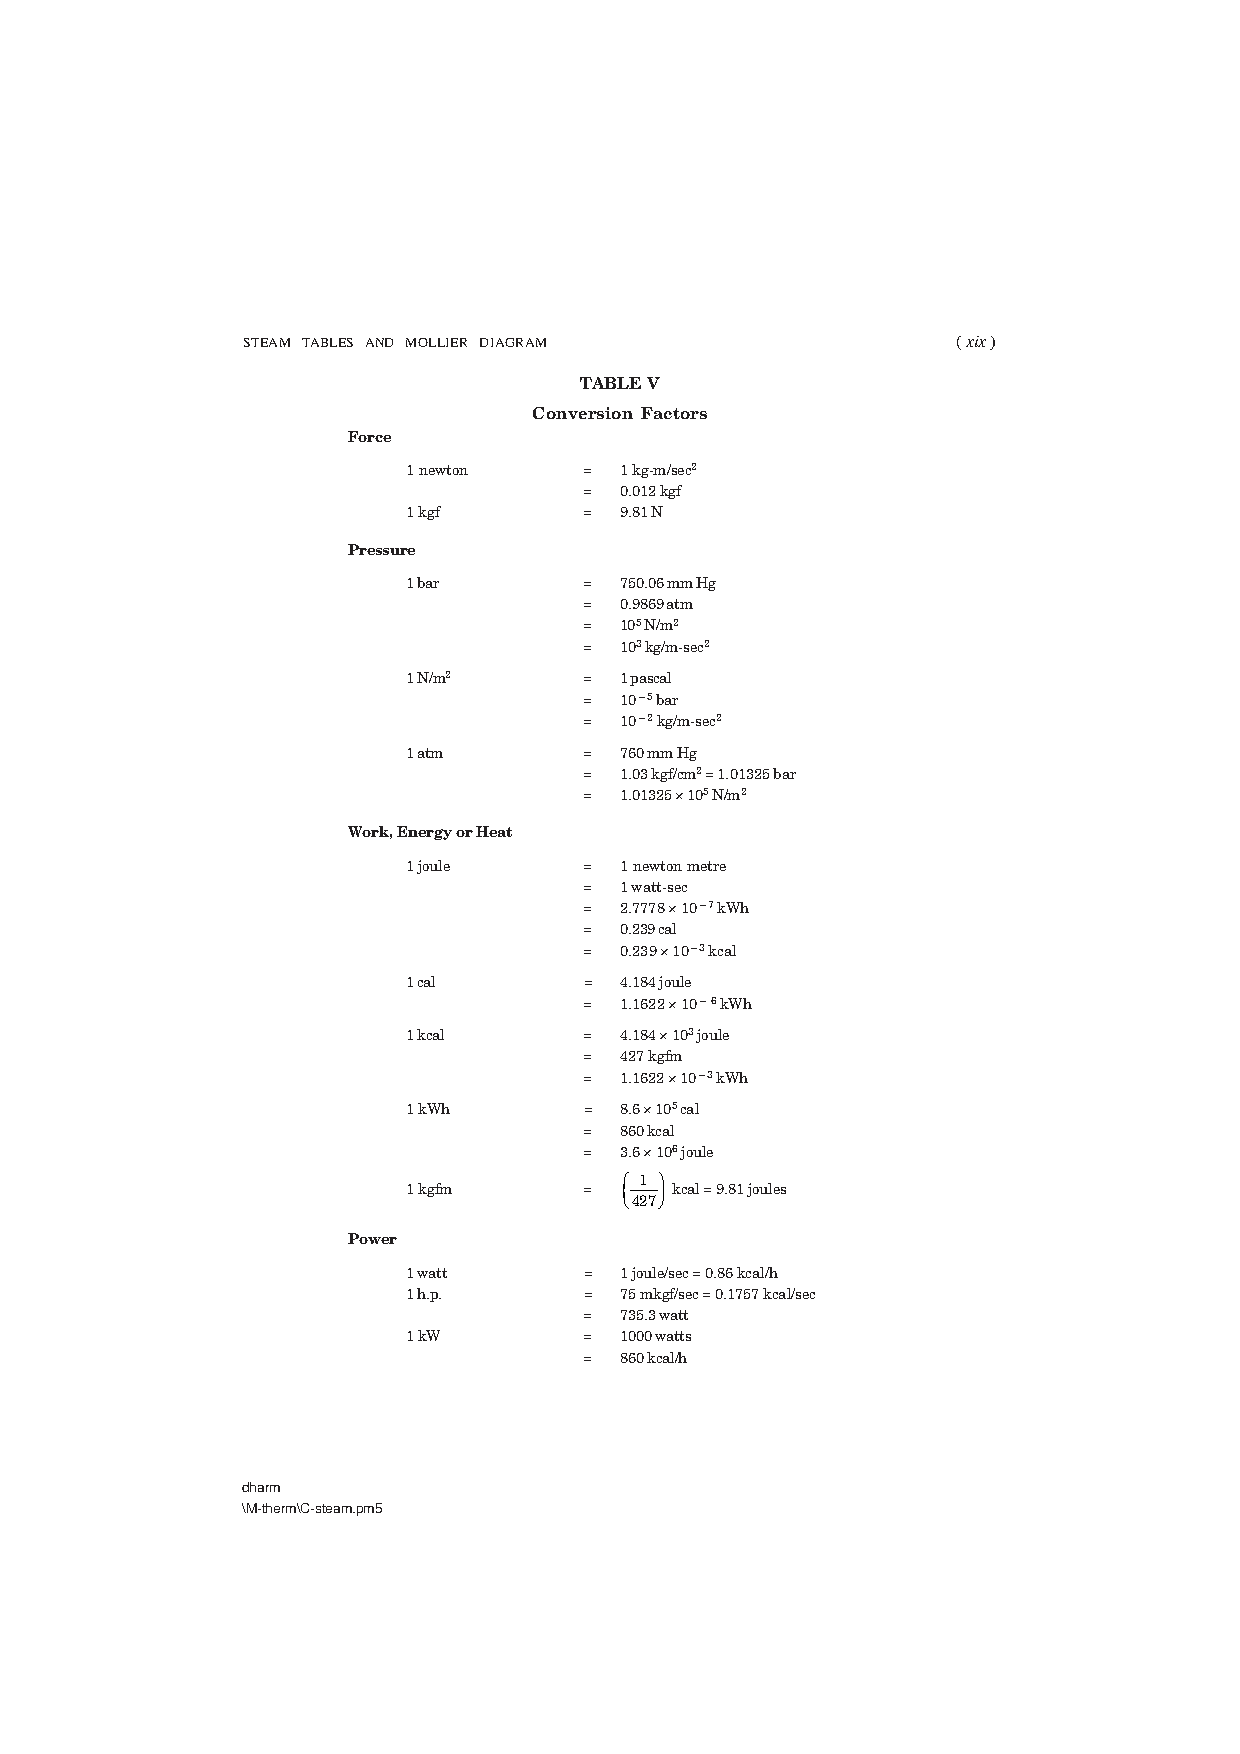
\includepdf[pages=-,fitpaper]{./UnitsConversion.pdf}
\includepdf[pages=-,fitpaper]{./SteamTable_2.pdf}
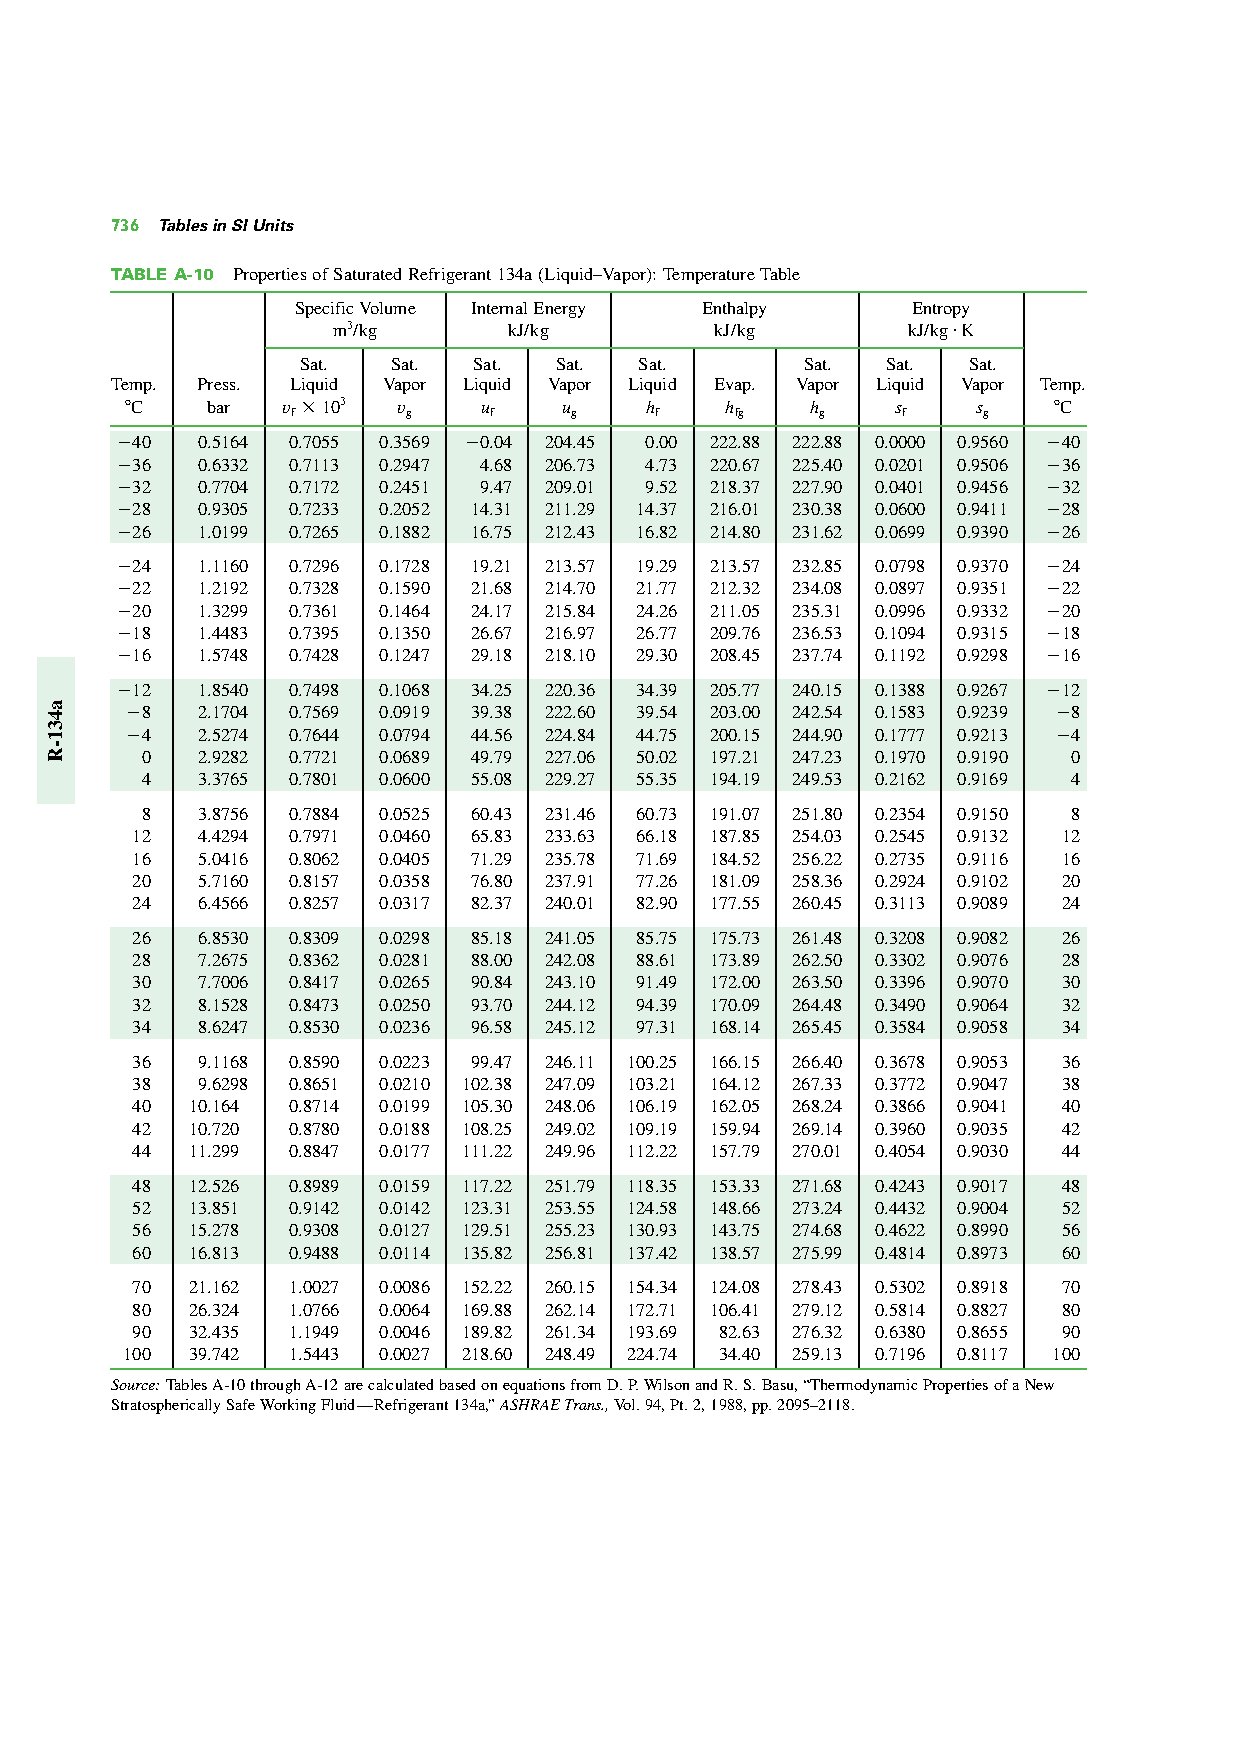
\includepdf[pages=-,fitpaper]{./Tables_R134.pdf}
\includepdf[pages=-,fitpaper]{./PsychrometricChart.pdf}
}


\vfill

\paperend
\end{document}
